\section{Inheritance and Polymorphism}
Inheritance enables a new class (subclass or derived class) to adopt the properties and 
methods of an existing class (superclass or base class).

\begin{minipage}{0.5\columnwidth}
    \begin{itemize}
        \item code reuse
        \item modularity
        \item and the establishment of an ``is-a'' relationship.
    \end{itemize}
\end{minipage}
\begin{minipage}{0.5\columnwidth}
    \begin{center}
        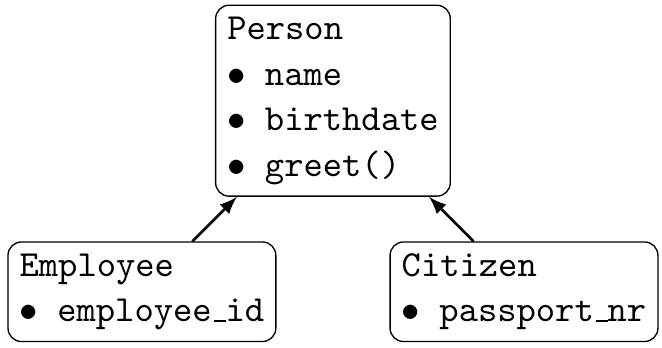
\includegraphics[width=\linewidth]{images/vererbung3.png}
    \end{center}
\end{minipage}\medskip
    
Polymorphism allows subclasses to define methods with the same name as those in the superclass, effectively overriding them. The specific method invoked depends on the actual object type at runtime, increasing interface flexibility.

\subsubsection{The \texttt{super()} Function}
The \texttt{super()} function provides access to methods and attributes of the superclass. It is primarily used within the subclass's \texttt{\_\_init\_\_} method to initialize inherited attributes, ensuring the proper setup of the base object state.

\begin{lstlisting}[language=Python]
class Person:
    def __init__(self, name):
        self.name = name

class Employee(Person):
    def __init__(self, name, employee_id):
        super().__init__(name) # Initialize superclass attributes
        self.employee_id = employee_id
\end{lstlisting}

\subsubsection{Abstract Classes}
Abstract classes serve as templates and cannot be instantiated directly. They define abstract methods that must be implemented by derived classes, enforcing a consistent interface. This requires the \texttt{abc} module.

\begin{lstlisting}[language=Python]
from abc import ABC, abstractmethod

class Vehicle(ABC):
    @abstractmethod
    def accelerate(self):
        pass

class Car(Vehicle):
    def accelerate(self):
        print('The car accelerates')
\end{lstlisting}

\subsection{Design Principles (SOLID)}
When constructing inheritance hierarchies, adhering to design principles ensures flexibility and maintainability:
\begin{itemize}
    \item \textbf{S}ingle Responsibility: A class should have only one responsibility and be responsible for exactly one thing.
    \item \textbf{O}pen-Closed: Classes should be open for extension (e.g., via inheritance) but closed for modification.
    \item \textbf{L}iskov Substitution: Objects of a superclass should be replaceable with objects of a subclass without affecting program correctness.
    \item \textbf{I}nterface Segregation: Clients should not be forced to depend on unused methods.
    \item \textbf{D}ependency Inversion: High-level modules should not depend on low-level modules; both should depend on abstractions.
\end{itemize}

\subsection{Aggregation and Composition}
Overusing inheritance can lead to a ``class explosion'' problem, significantly increasing 
complexity when combining multiple traits or options. 

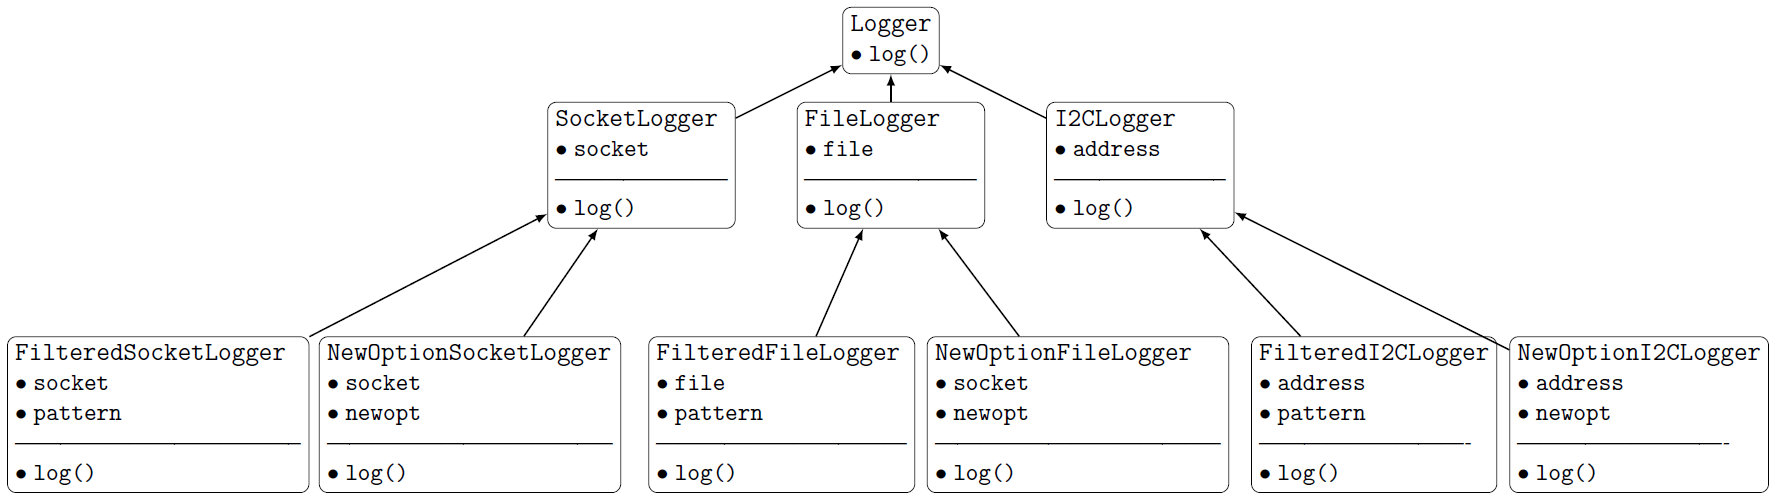
\includegraphics[width=\linewidth]{images/vererbung9.png}

Aggregation and composition offer 
structural alternatives by composing \textbf{classes based on dependencies rather than strict 
hierarchies.}\medskip

\begin{itemize}
    \item \textbf{Composition (is-a-part-of):} Implies a strong lifecycle dependency. The parent object owns and controls the lifetime of the contained objects. If the parent is destroyed, its parts are also destroyed (e.g., a Car and its Engine).
    \item \textbf{Aggregation (has-a):} Implies a loose lifecycle dependency. Contained objects can exist independently of the parent object and can be dynamically added or removed (e.g., a Library and its Books).
\end{itemize}

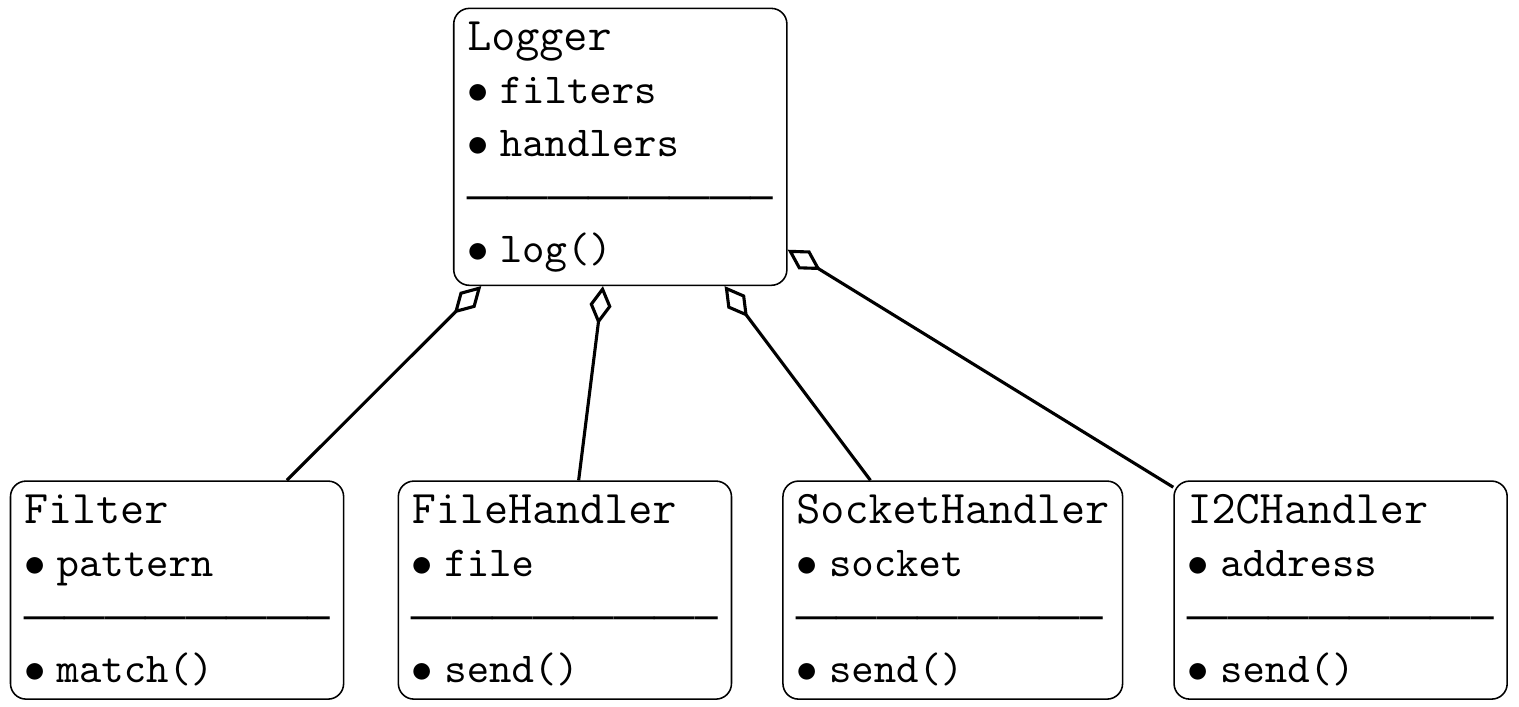
\includegraphics[width=\linewidth]{images/aggregation.png}

\lstinputlisting[language=Python]{code/aggregation.py}